\documentclass[11pt]{article}
\usepackage[paperwidth=8.5in, paperheight=11in]{geometry}
\usepackage{algorithm}
\usepackage{algorithmicx}
\usepackage[noend]{algpseudocode}

\usepackage{../tjimo}

\newcommand{\sevenpoints}{Time limit: 45 minutes.}
\newcommand{\righthead}{\fdbox{Round}{Power}}

\begin{document}

\section{What is a Graph?}

You might have heard of a graph in your math class as a plot with an $x$ and $y$ axis. Or maybe in science you looked at
bar graphs and pie graphs. Maybe in history you took a look at line graphs. But the graphs we are going to talk about today
are none of the above.

\subsection{Some Introduction}

At its core, a \textit{graph} consists of two sets: a group of objects, and a group of connectors that each join two objects.

To gain insight into what a graph is, let's first consider flights that connect airports around the world.
We depend on airplanes to travel quickly and efficiently. When we want to travel between major cities,
like between D.C. and Boston, we can often take a single flight to make the trip. Enough people want to travel between
these two cities for it to be economical to offer a single flight between them.

However, it is not always the case that single-flight trips are economically feasible, either due to lack of demand
or due to needing to refuel. To travel from London to Yellowstone, for example, one must first stop in Atlanta, hop
on a connecting flight to Denver, and then finally travel to Yellowstone. Denver and Atlanta are what we call
hubs, since they are very large airports that accomodate heavy travel loads. To travel between smaller airports, we often
need to stop at one of these larger hubs.

\begin{center}
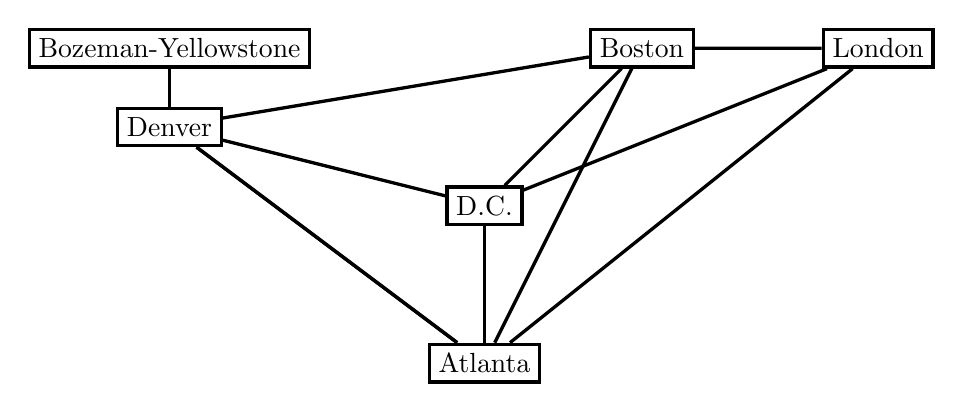
\begin{tikzpicture}[very thick,level/.style={sibling distance=70mm/#1}]
\draw (0, 0) node[draw, shape=rectangle] (a) {D.C.};
\draw (-4, 1) node[draw, shape=rectangle] (b) {Denver};
\draw (0, -2) node[draw, shape=rectangle] (c) {Atlanta};
\draw (2, 2) node[draw, shape=rectangle] (d) {Boston};
\draw (5, 2) node[draw, shape=rectangle] (e) {London};
\draw (-4, 2) node[draw, shape=rectangle] (f) {Bozeman-Yellowstone};
\draw (a) -- (b) -- (c) -- (d) -- (e);
\draw (b) -- (f);
\draw (c) -- (b);
\draw (a) -- (d);
\draw (b) -- (d);
\draw (a) -- (c);
\draw (c) -- (e);
\draw (a) -- (e);
\end{tikzpicture}
\end{center}

Our connections between our cities in the graph represent only direct connections between
cities, but from our diagram, we can still see it is possible to travel between any two
cities in our graph.

Neither the exact position of each city nor how connections might intersect 
matters. In other words, the way we draw a graph on paper does not change its properties, and for the most part
are not useful to us. The following is an equivalent graph:

\begin{center}
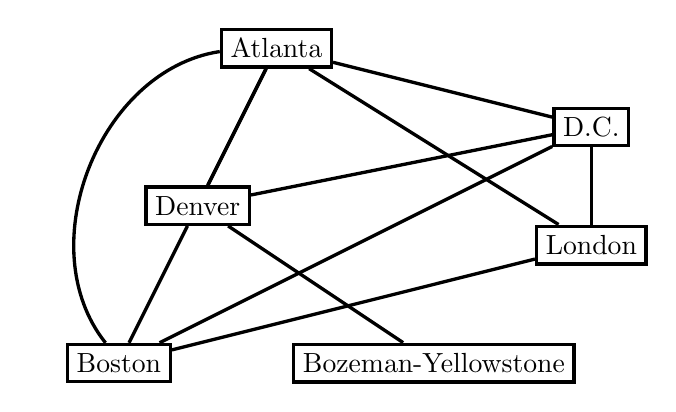
\begin{tikzpicture}[very thick,level/.style={sibling distance=70mm/#1}]
\draw (5, 3) node[draw, shape=rectangle] (a) {D.C.};
\draw (0, 2) node[draw, shape=rectangle] (b) {Denver};
\draw (1, 4) node[draw, shape=rectangle] (c) {Atlanta};
\draw (-1, 0) node[draw, shape=rectangle] (d) {Boston};
\draw (5, 1.5) node[draw, shape=rectangle] (e) {London};
\draw (3, 0) node[draw, shape=rectangle] (f) {Bozeman-Yellowstone};
\draw (a) -- (b) -- (c);
\path (c) edge [bend right=60] (d);
\draw (d) -- (e);
\draw (b) -- (f);
\draw (c) -- (b);
\draw (a) -- (d);
\draw (b) -- (d);
\draw (a) -- (c);
\draw (c) -- (e);
\draw (a) -- (e);
\end{tikzpicture}
\end{center}

The only characteristics of a graph we care about are the objects (in this case, cities) themselves, which we'll call \textit{vertices},
and the connections joining the objects, which we'll call \textit{edges}.

\subsection{Definition of a Graph}

We now have the background necessary to present the mathematical definition of a graph:

\begin{definition}
\label{def:graph}
A \textit{graph} $G(V,E)$ consists of a set of vertices $V$ and a set of edges $E$. 

\begin{center}
\begin{tikzpicture}[very thick,level/.style={sibling distance=70mm/#1}]
\draw (0, 0) node [vertex] (a) {$a$};
\draw (2, 1) node [vertex] (b) {$b$};
\draw (2, -1) node  [vertex] (c) {$c$};
\draw (4, 0) node [vertex] (d) {$d$};
\draw (a) -- (b);
\draw (b) -- (c);
\draw (c) -- (d);
\draw (b) -- (d);
\draw (a) -- (c);
\draw (6, -1) node [vertex] (e) {$e$};
\draw (6, 1) node [vertex] (f) {$f$};
\draw (8, 1) node [vertex] (g) {$g$};
\draw (8, -1) node [vertex] (h) {$h$};
\draw (e) -- (f) -- (g) -- (h) -- (f);
\draw (10, 0) node[vertex] (i) {$i$};
\draw (12, 0) node[vertex] (j) {$j$};
\draw (i) -- (j);
\end{tikzpicture}
\end{center}
\end{definition}

\begin{definition}
\label{def:edge}
An \textit{edge} is a collection of exactly two vertices. In the above graph, there is an edge
between $a$ and $b$, so $\{a, b\}$ is an edge. Note that $\{a,b\}$ is the same edge as $\{b,a\}$.
\end{definition}

\begin{definition}
\label{def:set}
A \textit{set} is a collection of any number of objects. In the above graph, we have the set of vertices
\[V=\{a, b, c, d, e, f, g, h, i, j\}.\]
We also have the set of edges
\[E=\{\{a,b\}, \{b,c\}, \{c,d\},\{b,d\},\{a,c\},\{e,f\},\{f,g\},\{g,h\},\{h,f\},\{i,j\} \}.\]
\end{definition}

\begin{definition}
\label{def:cardinality}
Given a set $A$, the cardinality $\abs{A}$ denotes the number of elements in $A$.
\end{definition}

\begin{problem} % problem 1
Evaluate $\abs{V}$ and $\abs{E}$ for the sets $V$ and $E$ in Definition \ref{def:set}, the definition of the set.
Note that $\{a,b\}$ counts as one single edge.
\end{problem}

\begin{solution}
Answer: $\abs{V} = \abs{E} = \boxed{10}$. \\
There are 10 vertices and 10 edges in the graph.
\end{solution}

\begin{problem} % 2
Draw any graph with 5 vertices and 8 edges.
\end{problem}

\begin{solution}
The following graph has 5 vertices and 8 edges.
\begin{center}
\begin{tikzpicture}[very thick,level/.style={sibling distance=70mm/#1}]
\draw (6, -1) node [vertex] (a) {$a$};
\draw (6, 1) node [vertex] (b) {$b$};
\draw (8, 1) node [vertex] (c) {$c$};
\draw (8, -1) node [vertex] (d) {$d$};
\draw (10, 0) node [vertex] (e) {$e$};
\draw (a) -- (b) -- (c) -- (d) -- (a) -- (c) -- (e) -- (d) -- (b);
\end{tikzpicture}
\end{center}
\end{solution}

\subsection{Graph Basics}

\begin{definition}
\label{def:degree}
The $degree$ of a vertex is the number of neighbors it has. For vertex $b$ in the following graph, we write $deg(b) = 3$,
meaning the degree of $b$ is 3.
\begin{center}
\begin{tikzpicture}[very thick,level/.style={sibling distance=70mm/#1}]
\draw (0, 0) node [vertex] (a) {$a$};
\draw (2, 1) node [vertex] (b) {$b$};
\draw (2, -1) node  [vertex] (c) {$c$};
\draw (4, 0) node [vertex] (d) {$d$};
\draw (a) -- (b);
\draw (b) -- (c);
\draw (c) -- (d);
\draw (b) -- (d);
\draw (a) -- (c);
\end{tikzpicture}
\end{center}
\end{definition}

\begin{problem} % 3
Show that the total number of edges in a graph is equal to
\[\frac{1}{2} \cdot \sum_{\text{all vertices $v$}} deg(v).\]
The symbol $\sum$ means add up $deg(v)$ over all vertices $v$. In the graph in Definition \ref{def:degree},
\begin{align*}
\sum_{\text{all vertices $v$}} deg(v) &= deg(a) + deg(b) + deg(c) + deg(d) \\
&= 2 + 3 + 3 + 2 \\
&= 10.
\end{align*}
\end{problem}

\begin{solution}
The degree of a vertex represents the total number of edges that include that vertex. When we sum all the degrees together,
we consider every edge in the graph twice, since each edge contributes to the degrees of two different vertices. Thus, the total number
of edges in the graph is equal to 
\[\frac{1}{2} \cdot \sum_{\text{all vertices $v$}} deg(v).\]
\end{solution}

\begin{definition}
\label{def:clique}
A \textit{clique} is a graph such that there is exactly one edge covering every pair of distince vertices in the graph.
We denote a clique of $n$ vertices as $K_n$.
Pictured is a clique of 4 vertices, or $K_4$.
\begin{center}
\begin{tikzpicture}[very thick,level/.style={sibling distance=70mm/#1}]
\draw (6, -1) node [vertex] (a) {$a$};
\draw (6, 1) node [vertex] (b) {$b$};
\draw (8, 1) node [vertex] (c) {$c$};
\draw (8, -1) node [vertex] (d) {$d$};
\draw (a) -- (b) -- (c) -- (d) -- (a);
\draw (a) -- (c);
\draw (b) -- (d);
\end{tikzpicture}
\end{center}
\end{definition}

\begin{problem} % 4
Solve each of the following:
\begin{enumerate}[label=(\alph*)]
\item How many edges are in the clique of 4 vertices, $K_4$?
\item How many edges are in the clique of 5 vertices, $K_5$?
\item In terms of $n$, how many edges are in the clique of $n$ vertices, $K_n$, where $n$ is any positive integer?
\end{enumerate}
\end{problem}

\begin{solution} 
The number of edges in a clique are as follows:
\begin{enumerate}[label=(\alph*)]
\item $K_4$ has \boxed{6} edges: $\{a, b\}$, $\{a, c\}$, $\{b, c\}$, $\{a, d\}$, $\{b, d\}$, $\{c, d\}$.
\item $K_5$ has \boxed{10} edges: $\{a, b\}$, $\{a, c\}$, $\{b, c\}$, $\{a, d\}$, $\{b, d\}$, $\{c, d\}$, $\{a, e\}$, $\{b, e\}$, $\{c, e\}$, $\{d,e\}$.
\item In general, $K_n$ has
\[\binom{n}{2} = \boxed{\frac{n \cdot (n - 1)}{2}}\]
edges. \\
We need to count the total number of possible ways to choose two different vertices from $n$ total vertices. We have $n$ ways to choose the first vertex
and $n - 1$ ways to choose the second vertex, but the order in which we choose the vertices doesn't matter (that is, $\{A,B\}$ represents the same edge
as $\{B, A\}$), so we must divide by 2 to get the correct answer of $\frac{n \cdot (n - 1)}{2}$.

Alternatively, we could have used the previous problem directly and plugged into our formula.
\end{enumerate}
\end{solution}

\section{Bipartite Graphs}

\begin{definition}
\label{def:bipartite}
A \textit{bipartite graph} is a graph whose vertices can be divided into two disjoint, or nonoverlapping, sets, $S$ and $T$, such that every
edge in the graph connects one vertex in $S$ to one vertex in $T$. The following is an example of a bipartite graph:
\begin{center}
\begin{tikzpicture}[very thick,level/.style={sibling distance=70mm/#1}]
\draw (-2, 0) node [vertex] (a) {$a$};
\draw (-2, -1) node [vertex] (b) {$b$};
\draw (-2, -2) node [vertex] (c) {$c$};
\draw (-2, -3) node [vertex] (d) {$d$};
\draw (2, 0) node [vertex] (e) {$e$};
\draw (2, -1) node [vertex] (f) {$f$};
\draw (2, -2) node [vertex] (g) {$g$};
\draw (2, -3) node [vertex] (h) {$j$};
\draw (2, -4) node [vertex] (i) {$i$};
\draw (a) -- (f);
\draw (a) -- (g);
\draw (b) -- (i);
\draw (b) -- (h);
\draw (c) -- (e);
\draw (c) -- (f);
\draw (c) -- (h);
\draw (d) -- (i);
\end{tikzpicture}
\end{center}
We can split the vertices into two sets: $S=\{a,b,c,d\}$ and $T=\{e,f,g,h,i\}$. Every edge in the graph connects a vertex in $S$ to
one in $T$. No edge connects two vertices from $S$, and no edge connects two vertices from $T$.
\end{definition}

\begin{problem} % 5
Given a graph $G$, three vertices $a$, $b$, and $c$ in the graph are such that an edge connects $a$ and $b$, an edge connects $b$ and $c$, and an edge
connects $c$ and $a$. Show that the graph $G$ cannot be bipartite.
\end{problem}

\begin{solution}
If $G$ were bipartite, then its vertices can be partitioned into exactly two sets such that the vertices in each set are not connected by an edge.
this means that $a$ and $b$ are in different sets, $b$ and $c$ are in different sets, and $c$ and $a$ are in different sets. however, this is not possible
with only two sets, so $g$ must not be bipartite.
\end{solution}

\begin{problem} % 6
As a result of the previous problem, bipartite graphs have no $K_3$. However, given a graph $G$ with no $K_3$, must it be bipartite?
\end{problem}

\begin{solution}
No. The following graph has no $K_3$, but is not bipartite.
\begin{center}
\begin{tikzpicture}[very thick,level/.style={sibling distance=70mm/#1}]
\draw (0, 1) node [vertex] (a) {$a$};
\draw (-0.951, 0.309) node [vertex] (b) {$b$};
\draw (-0.588, -0.809) node [vertex] (c) {$c$};
\draw (0.588, -0.809) node [vertex] (d) {$d$};
\draw (0.951, 0.309) node [vertex] (e) {$e$};
\draw (a) -- (b) -- (c) -- (d) -- (e) -- (a);
\end{tikzpicture}
\end{center}
If it were bipartite, $a$ would be in a different set as $b$, so it would be in the same set as $c$, and so on, meaning $a$ is in a different set as $a$, a contradiction.
\end{solution}

\begin{problem}
Let $n$ be an even integer. What is the maximum number of edges in a bipartite graph with $n$ vertices? Express your answer
in terms of $n$, and remember to explain your solution! You might find the following fact useful:
\begin{theorem}[AM-GM]
\label{thm:am-gm}
Given two nonnegative numbers $x$ and $y$,
\[\frac{x + y}{2} \ge \sqrt{x \cdot y}.\]
\end{theorem}
\end{problem}

\begin{solution}
Since the graph is bipartite, we can separate the graph into two sets, $S$ and $T$, such that $\abs{S} + \abs{T} = n$,
and no edges connect each set's vertices. The maximum number of edges in a graph separated into $S$ and $T$ is $\abs{S} \cdot \abs{T}$. However, by the
AM-GM Inequality,
\[\abs{S} \cdot \abs{T} \le \left(\frac{\abs{S} + \abs{T}}{2}\right)^2 \le \boxed{\frac{n^2}{4}}. \]
We see that this number of edges can be achieved by separating the $n$ vertices into two equally-sized sets.
\end{solution}

\section{Shortest Paths}

Graphs represent connections between different objects. We might, for example, have different cities connected in some way.
It takes a certain amount of time to get in between different neighboring cities. Perhaps to travel from D.C. to St. Louis,
we must either stop at Chicago or Cincinnati along the way. It might be faster to travel through Cincinnati, but it might be
cheaper to stop at Chicago. Either way, we need to devise some kind of system to determine for us the best way to travel between
vertices in our graph, through following some kind of \textit{path}.

\subsection{Introduction to Paths}

\begin{definition}
\label{def:path}
A \textit{path} is a sequence of vertices, such that every two consecutive vertices in the graph are connected by an edge.
All edges in the path must be distinct, and all the vertices must be distinct.
\end{definition}

\begin{problem} % 1
In the following graph, answer the questions below.
\begin{center}
\begin{tikzpicture}[very thick,level/.style={sibling distance=70mm/#1}]
\draw (6, -1) node [vertex] (a) {$a$};
\draw (6, 1) node [vertex] (b) {$b$};
\draw (8, 1) node [vertex] (c) {$c$};
\draw (8, -1) node [vertex] (d) {$d$};
\draw (a) -- (b) -- (c) -- (d) -- (b);
\end{tikzpicture}
\end{center}
\begin{enumerate}[label=(\alph*)]
\item Is $b,c$ a path?
\item Is $b,c,d$ a path?
\item Is $a,c,b$ a path?
\item Is $b,c,b$ a path?
\item Is $b,c,d,b$ a path?
\item Is $b$ a path?
\end{enumerate}
If your answer for any of these was ``no,'' explain why.
\end{problem}

\begin{solution}
From Definition \ref{def:path} of a path,
\begin{enumerate}[label=(\alph*)]
\item $b,c$ is a path.
\item $b,c,d$ is a path.
\item $a,c,b$ is not a path, since $a$ and $c$ are not connected.
\item $b,c,b$ is not a path, since $b$ is repeated.
\item $b,c,d,b$ is not a path, since $b$ is repeated.
\item $b$ is a path.
\end{enumerate}
\end{solution}

\subsection{Dijkstra's Shortest Path Algorithm}

In this subsection we explore an algorithm to compute the shortest, or cheapest, path from one vertex to another in a graph.
Thus, we'll want to assign some kind of value to each edge. For example, it might be the distance between two
vertices. We'll call this value the \textit{weight}.

\begin{definition}
\label{def:weight}
We assign to each edge $\{u,v\}$ a nonnegative \textit{weight} $w(u,v) \ge 0$. This is simply a number associated with the edge.
For example, it might represent the distance between $u$ and $v$ or the cost to travel between $u$ and $v$.
\end{definition}

Our main goal is to find a path from one vertex to another such that the sum of the weights along the path is
minimized. To travel along an edge in the path, we have to pay the weight of that edge.

\begin{definition}
\label{def:shortest-path}
Given a graph $G$, the \textit{shortest path} $v_0$, $v_1$, $v_2$, $v_3$, $\cdots$, $v_{m-2}$, $v_{m-1}$, $v_m$
from vertex $v_0$ to vertex $v_m$ is the path that minimizes
the sum
\[w(v_0,v_1) + w(v_1,v_2) + w(v_2, v_3) + \cdots + w(v_{m-2}, v_{m-1}) + w(v_{m-1}, v_{m}).\]
\begin{center}
\begin{tikzpicture}[very thick,edge from parent/.style={draw,<-},level/.style={sibling distance=30mm/#1}]
\draw (0, 0) node [vertex] (v1) {$a$};
\draw (1, 4) node [vertex] (v2) {$b$};
\draw (4, 1) node [vertex] (v3) {$c$};
\draw (5, 5) node [vertex] (v4) {$e$};
\draw (8, 3) node [vertex] (v5) {$d$};
\draw (v1) -- (v2) node[midway, left] {4};
\draw (v2) -- (v3) node[midway, above right] {2};
\draw (v1) -- (v3) node[midway, below] {7};
\draw (v2) -- (v4) node[midway, above] {6};
\draw (v3) -- (v4) node[midway, right] {3};
\draw (v3) -- (v5) node[midway, below] {5};
\draw (v4) -- (v5) node[midway, above] {4};
\end{tikzpicture}
\end{center}
In the above graph, the shortest path from $a$ to $e$ is $a$, $b$, $c$, $e$. The shortest, or cheapest,
distance from $a$ to $e$ is then 9. No other path can do better.
\end{definition}

\begin{problem} % 2
\label{example-computation}
Determine the shortest path and shortest-path length of each vertex from $a$. List the vertices in increasing order of the distance
from $a$ to that vertex.
\end{problem}

\begin{solution}
Shortest paths, in order: \\
$a$: $a$; length 0 \\
$b$: $a$, $b$; length 4 \\
$c$: $a$, $b$, $c$; length 6 \\
$e$: $a$, $b$, $c$, $e$; length 9 \\
$d$: $a$, $b$, $c$, $d$; length 11
\end{solution}

\begin{definition}
\label{def:source}
A \textit{source} is a vertex from which paths begin. In the above problem, $a$ was the source. Dijkstra's algorithm
is a single-source algorithm, which means it computes the shortest path from one source to all other vertices.
\end{definition}

\begin{problem} % 3
Let $u$ be a vertex immediately prior to vertex $v$ along the shortest path from source $s$ to $v$. Show that the shortest path from $s$ to $v$ must
pass along a shortest path to $u$ before traversing one final edge from $u$ to $v$.
\end{problem}

\begin{solution}
Suppose for the sake of contradiction that the path to $u$ along the shortest path to $v$ is not the shortest path. This means
there exists a path to $u$ shorter than the one along the path to $v$. But then there must also exist a shorter path to $v$, along
the shortest path to $u$ first and then along the edge from $u$ to $v$, which is a contradiction. Then the path to $u$ along the path to $v$
is a shortest path.
\end{solution}

Dijkstra's algorithm involves keeping track of a best known distance, which we'll call $dist(v)$ for each vertex $v$. Initially, $dist(v) = \infty$ for
all vertices $v$, except for the source $s$ of our graph, for which $dist(s) = 0$.

Then, if we were to run the algorithm on the example graph from before, the $dist$ of each vertex is as follows, at the very beginning:

\begin{center}
\begin{tabular}{ c | c }
vertex $v$ & $dist(v)$ \\
\hline
$a$ & 0 \\
$b$ & $\infty$ \\
$c$ & $\infty$ \\
$d$ & $\infty$ \\
$e$ & $\infty$ 
\end{tabular}
\end{center}

As we explore our graph, $dist(v)$ decreases, until $dist(v)$ represents the actual shortest-path distance from a source to $v$.

The way we explore the graph is we visit vertices one by one, in the order of closeness to the source, as you have computed in Problem \ref{example-computation}.
Therefore, the first vertex we visit is the source itself.

We only visit a vertex $v$ if we know for sure that the actual shortest-path distance to $v$ matches what we have stored in $dist(v)$.
When we visit $v$, we take a look at all vertices $u$ which share an edge with $v$. If $dist(v) + w(v,u) < dist(u)$, then we change the value of $dist(u)$
to be $dist(v) + w(v,u)$. In other words, we have explored enough of our graph to discover a path through $v$ to $u$ that is shorter than the one known up to that point.
This means that $dist(v)$, which is the best known distance thus far, also represents the best path to $v$ through all visited vertices.

Notice how, in the table below, $dist(b)$ and $dist(c)$ are updated, as they are neighbors of $a$, which was just visited.

\begin{center}
\begin{tabular}{ c | c | c }
vertex $v$ & $dist(v)$ & visited? \\
\hline
$a$ & 0 & yes \\
$b$ & 4 & no \\
$c$ & 7 & no \\
$d$ & $\infty$ & no \\
$e$ & $\infty$ & no
\end{tabular}
\end{center}

The vertex that has the minimum $dist$ that we haven't visited yet is $b$. Notice how $dist(c)$ and $dist(e)$ are updated in the table below, as they are neighbors of $b$.

\begin{center}
\begin{tabular}{ c | c | c }
vertex $v$ & $dist(v)$ & visited? \\
\hline
$a$ & 0 & yes \\
$b$ & 4 & yes \\
$c$ & 6 & no \\
$d$ & $\infty$ & no \\
$e$ & 10 & no
\end{tabular}
\end{center}

$dist(b) = 4$, which agrees with the actual shortest path distance to $b$.

\begin{problem} % 4
What is the next vertex we should visit? (Hint: which unvisited vertex has the minimum $dist$?)
Copy the table in your answer and update it so that three vertices are visited. Does $dist$ of this vertex agree with the actual
shortest path distance to it, as you computed in Problem \ref{example-computation}?
\end{problem}

\begin{solution}
The next vertex we visit should be $c$.
\begin{center}
\begin{tabular}{ c | c | c }
vertex $v$ & $dist(v)$ & visited? \\
\hline
$a$ & 0 & yes \\
$b$ & 4 & yes \\
$c$ & 6 & yes \\
$d$ & 9 & no \\
$e$ & 11 & no
\end{tabular}
\end{center}
$dist(c) = 6$, which agrees with the actual shortest path distance to $c$.
\end{solution}

What you should notice is that $dist(v)$ is the actual shortest distance to $v$ for all visited vertices $v$.

\begin{problem} % 5
Suppose that we have just visited $k$ vertices, where $k > 0$ is some positive integer. Furthermore, suppose that these $k$ vertices
are the $k$ closest of all the vertices to the source. Show that, of all the unvisited vertices, the vertex $v$ with the minimum $dist(v)$
is such that $dist(v)$ is equal to the actual shortest distance from the source to $v$. In other words, show that we can visit this vertex
and make it the $(k+1)$-th visited vertex.
\end{problem}

\begin{solution}
$dist(v)$ represents the best distance from the source to $v$ using only visited vertices. Suppose $dist(v)$ wasn't actually the least
distance from the source to $v$. Then the path must have gone through some unvisited vertex. Call that vertex $u$. However, we assumed $v$ to be the unvisited vertex
with the least $dist$, so $dist(u) \ge dist(v)$. However, this means the length of the path through $u$ is at least as long as $dist(v)$.
Therefore, $dist(v)$ must be equal to the least distance from the source to $v$.
\end{solution}

The previous problem allows us to continue to visit the closest unvisited vertex, until we have visited all the vertices. Once we finish visiting all the vertices,
$dist(v)$ will represent the shortest distance from the source to $v$. Dijkstra's algorithm in its entirety is outlined below!

\begin{algorithm}[H]
\caption{Dijkstra}
\begin{algorithmic}
\ForAll{vertices $v$}
	\State $dist(v) \gets \infty$ \Comment{This means set $dist(v)$ to be $\infty$.}
	\State $visited(v) \gets 0$ \Comment{This means set $visited(v)$ to be $0$.}
    \State $prev(v) \gets -1$ \Comment{This allows us to trace our path backwards to the source.}
\EndFor
\State $dist(src) \gets 0$ \Comment{Initialize the value of $dist$ for the source.}
\While{there exists a vertex $v$ such that $visited(v)=0$}
	\State Let $v$ be the vertex such that $visited(v)=0$ that minimizes $dist(v)$
    \State $visited(v) \gets 1$ \Comment{Visit the vertex.}
	\ForAll{neighbors $u$ of $v$}
    	\If{$visited(u) = 0$}
    		\State $alt \gets dist(v) + weight(v, u)$
			\If{$alt < dist(u)$}
				\State $dist(u) \gets alt$ \Comment{If we found a different path, update the value of $dist$.}
   	        	\State $prev(u) \gets v$
			\EndIf
        \EndIf
    \EndFor
\EndWhile
\end{algorithmic}
\end{algorithm}

Dijkstra's algorithm lets us comput the shortest or cheapest path from one vertex to another extremely quickly -- roughly on the order of the number of edges.
This means that even in a graph with 100,000 vertices and 100,000 edges a computer program can compute the shortest distance from one vertex to another in a fraction of 
a second! Perhaps in high school, you will code this up yourself and see it in action.

\section{Eulerian Circuits}

\begin{definition}
\label{def:eulerian-circuit}
A \textit{walk} is a sequence of vertices in which every pair of consecutive vertices is connected by an edge. Note that this is different from a path: walks are allowed
to repeat vertices.
\end{definition}

\begin{definition}
\label{def:eulerian-circuit}
An \textit{Eulerian circuit}, named after the Swiss mathematician Leonhard Euler, is a walk that begins and ends on the same vertex and traverses every edge in the
graph exactly once.
\end{definition}

\begin{problem}

\end{problem}

\subsection{Introduction to Cycles}

\subsection{Seven Bridges of K\"{o}nigsberg}

\end{document}
